\section{Motor driver block}

This section will describe in detail how the motor driver block receives a duty cycle and a direction, then uses these to generate and output a \textbf{PWM} signal according to the direction and speed set by the controller block.

\subsection{Description}

An easy way to visualize the inner workings is to divide the Motor Driver into two separate blocks. The first block’s task is to create a \textbf{PWM} signal which is equivalent to the duty cycle given by the controller. The second block’s task is to set the output of the \textbf{PWM} signal to the right pin on the H-Bridge in order to control the direction of the motor.

\subsection{Theory}

This section will describe the theories used for the implementation.

\subsubsection{PWM generation}

The \textbf{PWM} signal is created based on a looping counter and a threshold. Imagine a counter resetting whenever it reaches a certain value, creating a loop. If the value is set to the period of the wanted \textbf{PWM} signal and the \textbf{PWM} signal output is dependent on the counter value relative to a threshold, then you will be able create a looping output that is dependant on the threshold. Figure \ref{fig:PWMimplementationprinciple} shows an illustration of the behavior of \textbf{PWM} signal based on the looping counter and threshold.

\begin{figure}[h!]
	\centering
	\includegraphics[scale=0.5]{Billeder/PWMimplementationprinciple.png}
	\caption{ An example of a H-bridge }
	\label{fig:PWMimplementationprinciple}
\end{figure}

\subsubsection{H-bridge}
An H-bridge is a collection of 4 transistors, designed to control a DC motor. In figure \ref{fig:H-bridge} the concept is illustrated. When the red switches are on, the motor runs in one direction and vica versa for the blue switches. There are two H-bridges in the system, one for the pan motor and one for the tilt motor. For further information about H-bridges, consult the datasheet of the H-bridge in appendix \ref{sec:ContentonCD}.

\begin{figure}[h!]
\centering
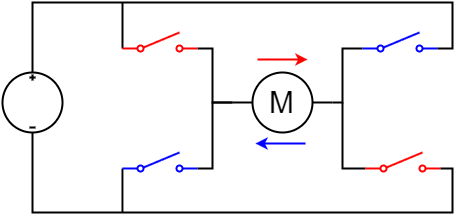
\includegraphics[scale=0.5]{Billeder/H-bridge.png}
\caption{ An example of a H-bridge }
\label{fig:H-bridge}
\end{figure}

\subsection{Implementation}

The implementation was done with the separation of the block described before. A \textbf{PWM} component was created which has the sole purpose of creating a \textbf{PWM} signal based on a duty cycle. The other part has the purpose of directing the \textbf{PWM} signal to the right output pins based on the direction wanted.

\subsubsection{PWM part}

The PWM block was implemented so that whenever the counter value is below the threshold the PWM signal output is high and when the counter value is above the threshold the PWM signal output is low. The section of the PWM code that makes the counter can be seen on picture \# Counting example \#.


\subsubsection{Direction part}

This block is simply implemented as a switch that toggles on the wanted direction. As an example if the wanted direction is set to 0 then the PWM is driven to the relevant motor control output and the other is kept at zero.

\subsection{Tests}

To verify that this motor controller is working as intended, a test bench was created and various inputs was tested. The enable was set and a duty cycle of 8 bits was input, which corresponds to a certain duty cycle. A clear spike in PWM output could be seen, of the same length every time PWM is outputting.
To further verify the test, the edges of the PWM signal was measured and used to find the exact duty cycle. Figure \ref{fig:MotorDriverTable} showcases the tests of PWM.

\begin{figure}[h!]
	\centering
	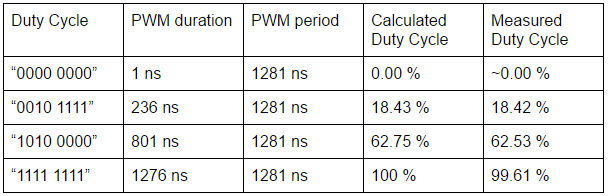
\includegraphics[scale=0.8]{Billeder/MotorDriverTabe.png}
	\caption{ PWM Tests }
	\label{fig:MotorDriverTable}
\end{figure}

\subsection{Discussion}

The tests show a deviation from the desired duty cycle of a small percentage. However these deviations have been deemed insignificant. The errors are created by the method that is used to calculate the PWM from the duty cycle. When converting the bit string, it is multiplied by the PWM period and divided by 256. This yields an integer, that when combined with the counter, yields a PWM very close to the desired duty cycle. Beyond that margin of error, a single clock cycle is lost due to resetting the counter, which corresponds to 1ns.


\subsection{Conclusion}

The motor driver has been sufficiently explained and tested, and has become a solid module to create a PWM signal for the P \& T system. The PWM calculation can be optimized very slightly by improving the conversion from duty cycle to PWM, and optimizing the counter, as to never lose any clock cycles.
